\section{Abstract}

The grouping of sound components across frequency and time is crucial for auditory scene analysis. When presented with ABA- pure tone sequences, subjects will report either hearing an integrated triplet pattern with a galloping rhythm, or report fission of the auditory sequence into two distinct isochronous streams. The strength of these perceptual organizations depends on the separation in frequency between tones as well as the presentation rate. These psychophysical effects are thought to reflect more general mechanisms for the brain to perform sequential streaming, for instance, grouping a series of footsteps together into one a representation of a single mover. We have developed a neuronal model which relates the strength of the cues for the integrated perceptual organization to the sensory coding of the stimulus itself. This model acts as a sequence detector, rapidly organizing incoming stimuli by recognizing underlying pattern regularities in the input. Our model uses the architecture of a synfire chain composed of Wilson Cowan neuronal units with persistent activity, and captures the temporal coherence boundary stimulus parameters for which fission of the grouped auditory percept's triplet pattern occurs. Because of the persistent activity inherent in bursting like Wilson Cowan (and Morris Lecar) neuronal dynamics, this model is resistant to the silent interval and gaps between tones, recognizing not just short term dependencies between subsequent auditory events but rather the global structure of the integrated tone pattern. We propose that such sequence detectors rapidly form and compete with one another in the case of ambiguous auditory inputs. The present work relates to previously reported psychophysics, human physiology eg mismatch negativity, and our own models for the case of perceptual bistability and buildup (Steele, Rinzel, Tranchina, 2012). Together, our computational models provide an account for the neuronal computations underlying the perceptual phenomenology of auditory scene analysis.

\section{
Introduction 
} 
\subsection{Experimental paradigm}
To form representations of sound sources in the environment, the auditory system can group incoming sound features across time and frequency. We use a sequence of pure tones in an ABA- pattern (van Noorden, 1975) for which observers typically report hearing either integration, with the tones grouped into triplets with a galloping rhythm, or segregation, in which the A and B tones are in separate streams with distinct rhythms. Psychophysical studies have shown that the perception of the ABA- tone sequence depends on the difference in frequency between tones, DF, time between subsequent tones T, and time since the beginning of the sequence presentation. Previous work (Steele et. al., 2012) has shown how buildup in probability of segregation can arise as a consequence of competition between
perceptual organizations. Here we propose a mechanistic model of how such organizations could be formed, and how they depend on stimulus parameters.

The model proposed here confers sequence selectivity through a syn-fire architecture, in which the response to each tone facilitates the response of the neurons tuned for the second tone. In order for the circuit to complete, the tones must be delivered in the right order. Neurons displaying sequence / interval selectivity have been found in the secondary auditory cortex (can i cite chia jung? marmosets?) belt and parabelt regions, and receive afferents from A1 (cite?). 

\subsection{Model objectives}:
\begin{itemize}
\item capture dependence of integrated percept on stimulus parameters DF and T
\item alternations should occur for intermediate DF
\item probability of segregation should increase over time in a stimulus-dependent fashion
\end{itemize}

\subsection{Previous approaches}

Rankin et al 2015 \cite{Rankin2015} Previous work from our lab has explored the issue broadly-
Like our model here, it has inputs that vary in time, pulsatile like tone responses.
It also has slow NMDA recurrent excitation for the gap.

Mill, Denham et al- Chains model, collisions. 
Model discovers repeating patterns in coded auditory features which then compete when there are collisions- when more than one repeating pattern predicts the same auditory feature/event.
[note - can we think of a neuromechanistic way to achieve this? we have to solve the A neuron problem anyway...]



Jin 2004 synfire- spiking model that recognizes very rapid (40 ms) sequences of inputs



Humble, Denham et al- network that learns sequences; employs global competition



May, Titiinen auditory cortex performs temporal integration


Anatomical/physiological evidence- probably in secondary auditory cortex and beyond; belt/parabelt regions
from james:
 Imaging studies have shown activation of a thalamocortical network [22] and the cerebellum [23] around the time of perceptual switches and an MEG study [18] localised to auditory cortex implicates non-primary auditory areas in maintaining perceptual streams.
Kondo & Kashino, thalamocortical loop in spontaneous switching (fMRI?)
Kashino, Kondo, Functional brain networks undertlying switching - streaming and verbal transformations

 Gutschalk, Micheyl, Melcher, Rupp, Scheg, Oxenham (!) Neuromagnetic correlates of streaming in human AC


\section{Methods}: 
Wilson-Cowan type firing rate neuronal populations with recurrent NMDA synapses and fast and slow inhibitory neurons, disinhibition type circuit

Present 3 spatially distinct input currents in order, scrambled, and at different speeds. The final neuron in the sequence - the 'output neuron' - will only fire in the case where the tones are presented in the correct order.

% \begin{figure}
% 	\centering
% 	\includegraphics[scale=.8]{ch4Figs/synfire_architecture_units.eps}
% 	\caption{The synfire architecture. A1 has a lower threshold (ie, perhaps a faster membrane time constant) and also creates a suppressive field }
% 	\label{fig:tooslow}
% \end{figure}\begin{figure}
% 	\centering
% 	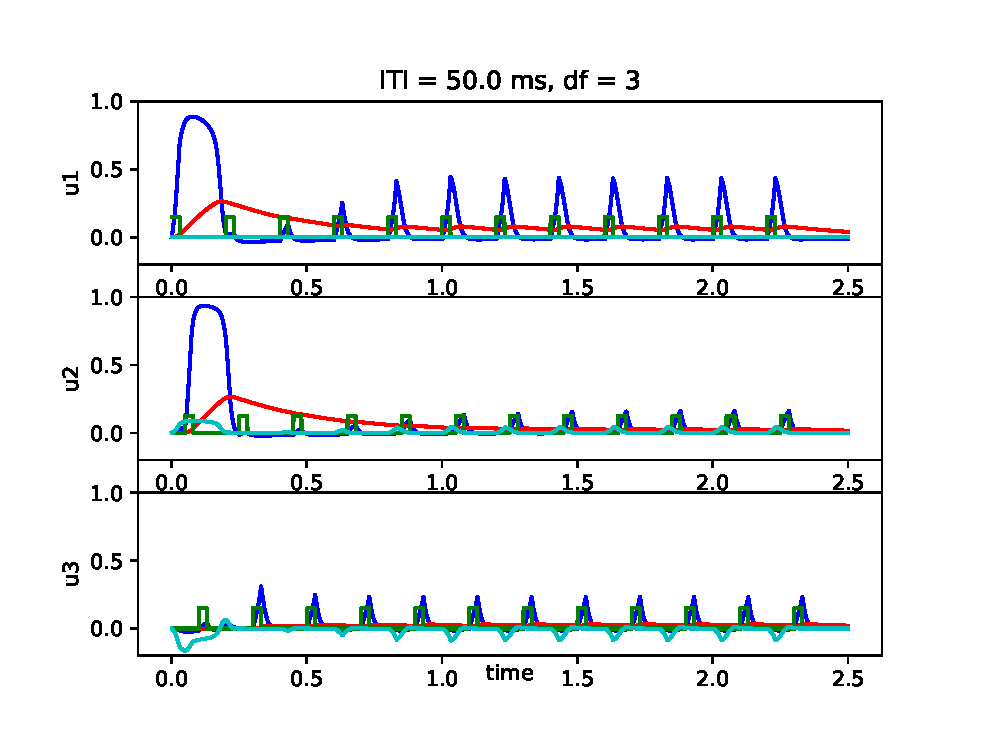
\includegraphics[scale=.8]{ch4Figs/sfa_wc_pop_func_50msITI_df3.eps}
% 	\caption{When tones are presented too fast, there is not enough time to recover from the lateral inhibition (forward suppression?)}
% 	\label{fig:tooslow}
% \end{figure}

methods:

3 wilson cowan units (morris lecar in supplemental) representing populations of auditory frequency-selective neurons, all have a best frequency of A. There is a simple tuning curve that describes the relationship between difference in frequency between A and B and the contribution of the B tone to the units.

the A units differ in their initial threshold- (i wonder if something similar can be accomplished with timescales...)

% Activation function:
% \frac{1}{(1 + \exp(-(x-\theta)/k)} - \frac{1}{(1 + exp(\theta/k))}

% with $k = .1$, $\theta = .3$

% Excitatory response and adaptation; first unit excites the second and suppresses the third. < can i write a function that makes this suppressive field? i think a normal "mexican hat" synaptic footprint between units would have the opposite weights - A would potentiate A and suppress B... let it go for now><back again - what if it potentiated A_highthresh so much that they all fired at the same time? then A couldn't fire again if presented super quickly... "refractoriness">

 Synaptic current (Isyn), firing rate (E) and adaptation defined by following equations for each unit receiving inputs from other units with weights $w_{i,j}$:

% weights_{i,j}

\begin{equation}
  \dot{Isyn} /dt = w_{ij}  
\end{equation}
% 

\cite{Ermentrout1997} neural nets as spatio-temporal pattern forming systems
" let i and j be the indices of two neurons which are connected such that the axon of neuron j terminates on the dendrite of neuron i
% voltage v_i turns into firing rate u_i(t) through activation function s(v_i(t))




Preliminary results:

\begin{figure}
	\centering
	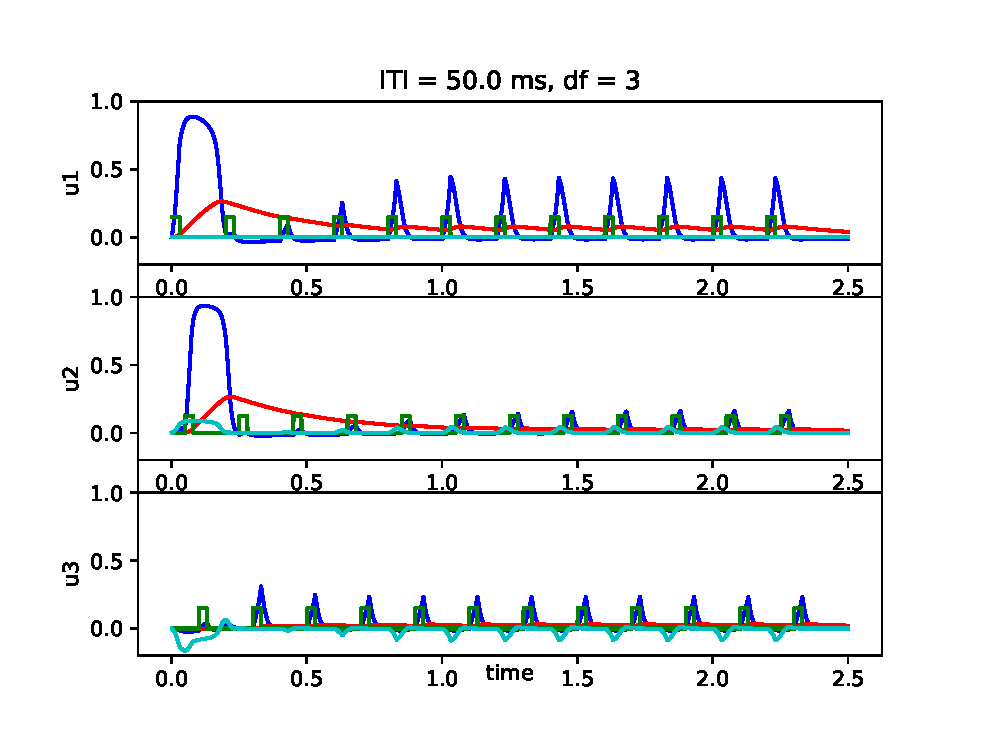
\includegraphics[scale=.8]{ch4Figs/sfa_wc_pop_func_50msITI_df3.eps}
	\caption{When tones are presented too fast, there is not enough time to recover from the lateral inhibition (forward suppression?)}
	\label{fig:tooslow}
\end{figure}

Can confer sensitivity to DF and timing interval over a reasonable range of stimulus and circuit parameters
Separate inputs; got to try the same thing for repeating inputs.
Future:
Try to have tonotopic layer feed into a temporal pattern layer
Further explore idea of synaptic depression conferring sequence selectivity
Use ingredients of inclusion and exclusion to produce collisions ideal proposed by Winkler


Concluding remarks:
This is a good framework for going from sensory coding to understanding phenomenology of the perceptual organization of sound
Improves existing algorithmic models with neuromechanistic processes

Future directions:

One of the issues with this approach conceptually is u1 and u3 here being tuned to the same frequency - why doesn't u3 get stimulated by the initial A tone?

Another issue is the question of the forward suppression between u1 and u3. Is it realistic that this neural population would maintain such a long and active inhibitory connection to neurons tuned to the same frequency? A typical "mexican hat" connection profile used in other works involving perceptual grouping and sensory integration \cite{Marti2013a} would suggest the opposite configuration- neuronal populations tuned to similar features recurrently excite one another, and suppress those tuned to dissimilar features. A third question is why the threshold is so much lower for u1. 
I believe a more elaborate architecture that accounted for both the dynamics of the A1 inputs and differences in time constants and tuning profiles between "sensory" neurons and "integration" neurons could achieve the same behaviors achieved by this model. The effect of the suppressive synapse from u1 to u3 would be replaced by attenuated A1 responses (ie \cite{Micheyl2005}, \cite{Micheyl2007} ; this suppressive synapse really just represents the forward suppression in A1 neurons recovering from a stimulus. 
We can replace the effect of the difference in thresholds by creating layers of tonotopic neuronal populations with a 'reservoir of time constants' - u1, receiving a narrow projection of a1 inputs in a skinny mexican hat, has a small (population) membrane time constant and a rapid response, whereas u2 and u3 have large membrane time constants and a wide connection profile. The two populations are also recurrently connected with a broad footprint- fast and slow neurons of one frequency stimulate the fast and slow neurons of nearby, but distinct, frequencies. The fat neurons require more sustained inputs to go off and can be thought of as 'integration' neurons.